\documentclass[../dissertation.tex]{subfiles}

\begin{document}
\begin{figure}[tpb]
    \centering
    \begin{subfigure}[b]{0.4\textwidth}
        \centering
        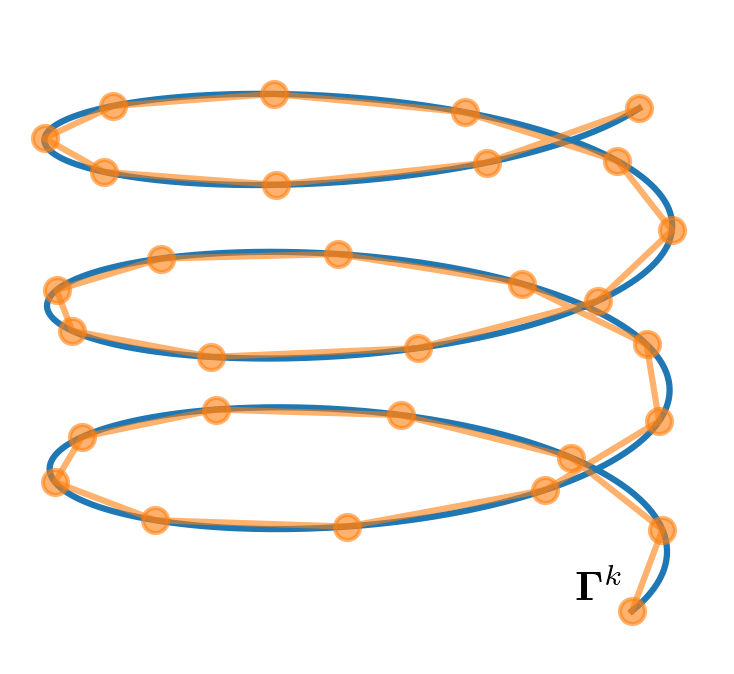
\includegraphics[width=\textwidth]{sections/otherHomeomorphismImgs/linesegment}
        \caption{A helix is an example of a curve homeomorphic to a line segment, so is in $\mathbb{L}$. Another notable curve in this class is a trefoil.}
        \label{fig: Line Segment Homeomorphism Class}
    \end{subfigure}
    \hspace{1cm}
    \begin{subfigure}[b]{0.4\textwidth}
        \centering
        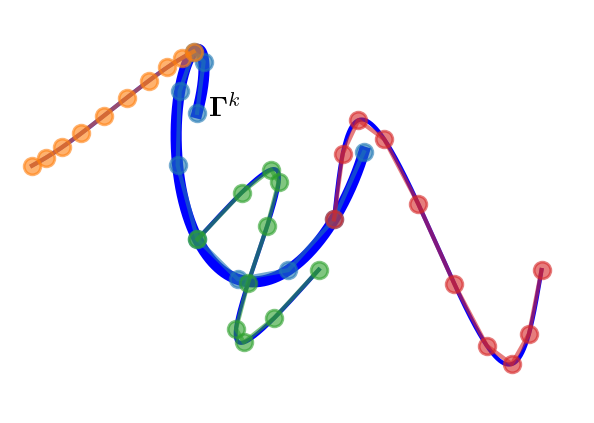
\includegraphics[width=\textwidth]{sections/otherHomeomorphismImgs/branch}
        \caption{A curve with 3 branches from a main ``stem''. This curve is homeomorphic to some tree, so is in $\overline{\mathbb{L}}$.}
        \label{fig: Bus Network}
    \end{subfigure}
    \caption{Curves in different homeomorphism classes.}
\end{figure}
Because homeomorphism relation is an equivalence relation, one could define equivalence classes.
We will call them homeomorphism classes.
\textit{We restrict our discussion to bounded curves.}

To make notation more concise, we introduce some labels:
\begin{itemize}
    \item Write $\mathbb{S}$ for the equivalence class of curves that are simple and closed; in other words, curves homeomorphic to a unit circle.
    \item Write $\mathbb{L}$ for the equivalence class of curves that are homeomorphic to a line segment.
    \item Write $\overline{\mathbb{L}}$ for the union of equivalence classes for curves that are homeomorphic to a tree graph, or a ``bus network''.
\end{itemize}

We have defined tangent-point energy quadrature for $\gammabf \in \mathbb{S}$ at (\ref{equ: Tangent-Point Energy Quadrature}).

For curves in different homeomorphism classes,
one may make minor changes to (\ref{equ: Tangent-Point Energy Quadrature}) to get a sensible quadrature.

Note that because curves in $\mathbb{L}$ and $\overline{\mathbb{L}}$ may have boundaries unlike curves in $\mathbb{S}$.
For the gradient operators derived in section \ref{sct: Gradient on Integer Sobolev Spaces} to be applicable, one assumes natural boundary conditions;
where the boundary integrals in lemma \ref{lemma: Shifting Gradient Operator} and \ref{lemma: Shifting Laplacian Operator} to be zero for any $g$ appropriate.
\subsection{Curves in $\mathbb{L}$}
\label{sct: Curves in L}
Given a curve $\gammabf \in \mathbb{L}$ such as the helix (Figure \ref{fig: Line Segment Homeomorphism Class}),
one could take the following as its tangent-point energy quadrature for its discretisation $\Gammabf^k$:
\begin{equation}
    E_{\beta}^{\alpha} \left( \Gammabf^k \right) \coloneqq \sum_{\substack{i,j \in \left\{ 1, \cdots, N-2 \right\} \\ r\left( i-j,N \right) > 1}} K_{\beta}^{\alpha} (i,j) \norm{e_i} \, \norm{e_j}
\end{equation}
where the contribution from each end is neglected.
Note that unlike a curve from $\mathbb{S}$
one need not generalise the indexing rule to be ``cyclic''.

\subsection{Curves in $\overline{\mathbb{L}}$}
For a curve $\gammabf \in \overline{\mathbb{L}}$ that has $m$ ``branches'' from a single ``stem'', one needs to take into account of at what points on the discretisation branching happens.
Suppose for all branches protrude from the stem.
On Figure \ref{fig: Bus Network}, the stem is represented by the thick blue curve.

One can capture this curve by an array of the following form.
\begin{equation}
    \Gammabf^k = \left( \underbrace{\xbf_{0,0}^k, \cdots, \xbf_{0,n_0-1}^k}_{\text{Stem}} \middle|
    \underbrace{\xbf_{1,0}^k, \cdots, \xbf_{1,n_1-1}^k}_{\text{Branch 1}}
\middle| \cdots \middle|
\underbrace{\xbf_{m,0}^k, \cdots, \xbf_{m,n_m-1}^k}_{\text{Branch } m}\right)
\label{equ: Bus Network Array}
\end{equation}
where the ``linkage points'' for branches to the stem are $\xbf_{1,0}^k, \cdots, \xbf_{m,0}^k$,
which can be identified by the fact that $\xbf_{1,0}^k, \cdots, \xbf_{m,0}^k \in \left\{ \xbf_{0,0}^k, \cdots, \xbf_{0, n_0-1}^k \right\}$,
that is, all duplicate points are to be understood as linkage points.
Denote the multiset\footnote{``a set that allows multiplicity of same elements''} of linkage points as $L \left( \Gammabf^k \right)$.
Then one may note the relation $N = \sum_{i=0}^{m} n_{i} - |L\left( \Gammabf^k \right)| = \sum_{i=0}^m n_i - m$.
Note that this is a natural generalisation for curves in $\mathbb{L}$.

Now, one may write a tangent-point energy quadrature as:
\begin{equation}
    E_{\beta}^{\alpha} \left( \Gammabf^k \right) \coloneqq 
    \sum_{p, q \in \left\{ 0, 1, \cdots, m \right\}}
    \sum_{\substack{
            i \in \left\{ 1, \cdots, n_p - 2 \right\} \\
            j \in \left\{ 1, \cdots, n_q - 2 \right\} \\
            \sigma \left( e_{p_i}, e_{q_j} \right) = 1
    }}
    K_{\beta}^{\alpha} (p_i,q_j) \norm{e_{p_i}} \, \norm{e_{q_j}}
    \label{equ: Bus Network Quadrature}
\end{equation}
where $p_i$ (similarly with $q_j$) refers to the index of vector $\xbf_{p,i}^k$ in (\ref{equ: Bus Network Array}),
that is,
\begin{align*}
    p_i = \sum_{j=0}^{p-1} n_j + i
\end{align*}

and
\begin{equation*}
    \sigma \left( e_1, e_2 \right) =
    \begin{cases}
        0 & \exists \text{ shared vertex between edges } e_1, e_2 \\
        1 & \text{Otherwise}
    \end{cases}
\end{equation*}

\begin{remark}
    Representation (\ref{equ: Bus Network Array}) is \textbf{not unique}; for example, one could take different curve to be the ``stem''.
    The quadrature given by (\ref{equ: Bus Network Quadrature}) is, however, invariant under different representation, hence well-defined.
\end{remark}


\subsection{General Curves: Loops and Trees}
One may now attempt to generalise to curves consisting of both closed loops (as in $\mathbb{S}$),
and trees (as in $\overline{\mathbb{L}}$).

While it is possible to write down the generalised quadrature,
but it may be more practical to summarise the strategy to build one.
\begin{enumerate}
    \item Identify the ``vertices''.
    \item Take an (ordered) pair of points on the discretised curve except for the points at boundary (that is, end of the branches or stems).
    \item Take two separate edges that involve the two points, but only one each.
        If the two edges share a vertex, disregard.
    \item Sum $K \norm{e_i} \, \norm{e_j}$ over all the pair of points chosen.
\end{enumerate}
\end{document}
